\chapter*{Results}

\section{Start}

\begin{table}[h]
    \caption{Instrument resolution function}
    \centering
    \begin{tabular}{|c|c|c|}
        \hline
        FWHM (ps) &  Shift (ps) & Intensity (\%) \\
        \hline
        213.3 & 0 & 80\\ 
        150 & -5 & 10\\ 
        267 & 17 & 10\\  
        \hline
    \end{tabular}
    \label{tab:irf}
\end{table}

\begin{figure}[h]
    \centering
    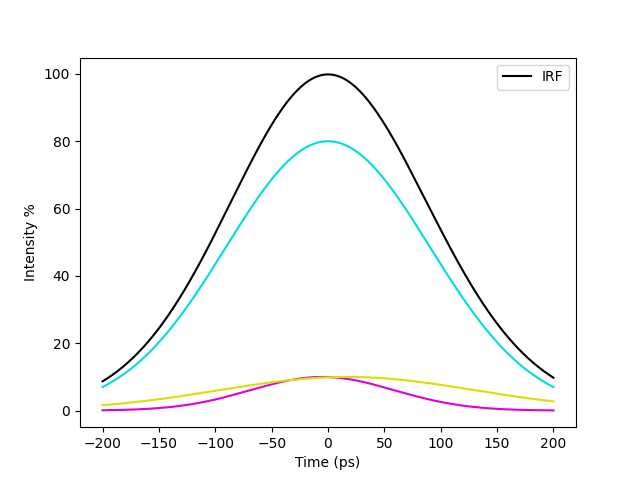
\includegraphics[width=0.8\textwidth]{Batch 3/regular IRF/irf.png}
    \caption{instrument resolution function}
    \label{fig:irf}
\end{figure}

Using PALSSIM, a series of spectra containing two positron lifetimes, $\tau_1$ and $\tau_2$, were generated with a three gaussian instrument resolution function (see Table \ref{tab:irf} and Figure \ref{fig:irf}). $\tau_1$ was kept fixed at 180ps and $\tau_2$ varied from 220-280ps, in 10ps intervals. For each value of $\tau_2$, three spectra were generated with the relative intensities of $\tau_1$ and $\tau_2$ set to 20\%-80\%, 50\%-50\% and 80\%-20\%. All the resulting spectra were then analyzed using PALSFIT, in order to evaluate how well the program could extract the two lifetimes, and their respective intensities, from each simulated spectrum.

In Figure \ref{fig:180-tau1}, we can observe how the values of $tau_1$ outputted by the program change, as the simulated value of $tau_2$ (on the horizontal axis) increases and the relative intensities (indicated by color and shape of marker) vary. Zooming in to the $\tau_2$ = 250-270ps range, we can see in Figure \ref{fig:180-tau1-zoomed} that, for these values in particular, PALSFIT struggles to determine $\tau_1$ in the 50-50 and 80-20 case. 

When evaluating $\tau_2$, unlike with $\tau_1$ where the simulated value of the lifetime was kept fixed, as the simulated value of the second lifetime changes, the difference between the result and the original values of $\tau_2$ is plotted in Figure \ref{fig:180-tau2}. In the figure we can see that, aside from the 20-80 spectrum for $\tau_2$ = 220, the software performs better than for $\tau_1$.

The error bars represent the standard deviation of -- and thus the confidence of the program in -- the lifetimes. From them, we see two factors that affect the size of the bars. The first is the relative intensities of the two intensities. In fact, in Figure \ref{fig:180-tau1}, which plots $\tau_1$, the error bars are the smallest for the 80-20 data, where the shorter lifetime is more intense, and in Figure \ref{fig:180-tau2}, tracking $\tau_2$, the opposite is the case and we have the 20-80 data is most precise. Observing all the figures, we see the second factor: as the time interval between the two lifetimes increases, the size of the error bars decrease.

In Figures \ref{fig:180-2080} - \ref{fig:180-8020} the fitted intensities of the two lifetimes are plotted against simulated $\tau_2$, for each combination of simulated intensities. In the figures, we see that when the relative intensity of $\tau_2$ was greater or equal to $\tau_1$, then PALSFIT was able to calculate all the appropriate lifetime intensities. However, when the intensity of $\tau_2$ was set to 80\%, shown in Figure \ref{fig:180-2080}, the software was unable to output the correct intensities for the first two simulated values of $\tau_2$. Looking at our error bars, we can see the same relationship between their size and the lifetime separation mentioned earlier.

On the whole, PALSFIT seems to have performed well, but not perfectly. As the first lifetime, $\tau_1$, was kept constant at 180ps, the next step would be to change $\tau_1$ and see how that affects our results. 

\todo{expand paragraph}

\begin{figure}[p]
    \caption{}
    \centering
    \makebox[\linewidth][c]{
        \begin{subfigure}{0.7\textwidth}
        \centering
        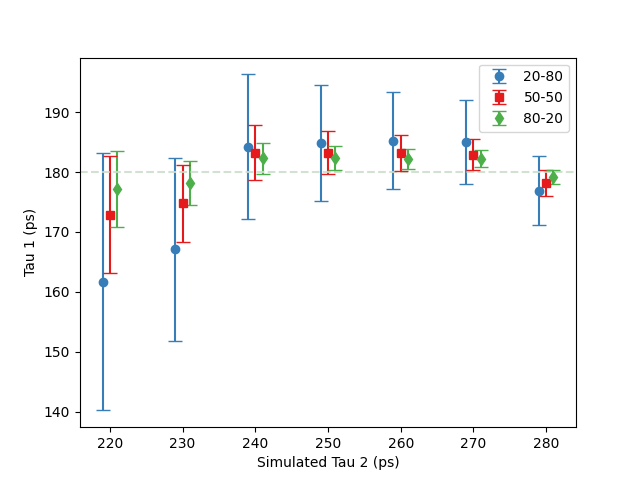
\includegraphics[width=0.95\linewidth]{Batch 1+2/t1.png}
        \caption{fixed $\tau_1 = 180ps$}
        \label{fig:180-tau1}
    \end{subfigure}
    \begin{subfigure}{0.7\textwidth}
        \centering
        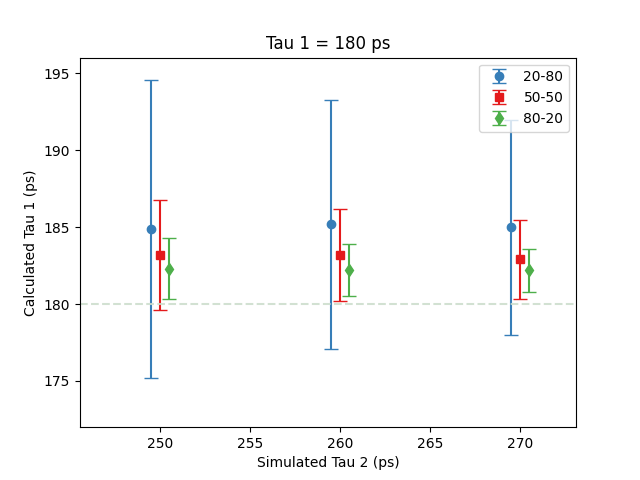
\includegraphics[width=.95\textwidth]{Batch 1+2/Tau1 stragglers.png}
        \caption{close-up $\tau_1 = 180ps$}
        \label{fig:180-tau1-zoomed}
    \end{subfigure}
    }
    \makebox[\linewidth][c]{
    \begin{subfigure}{0.7\textwidth}
        \centering
        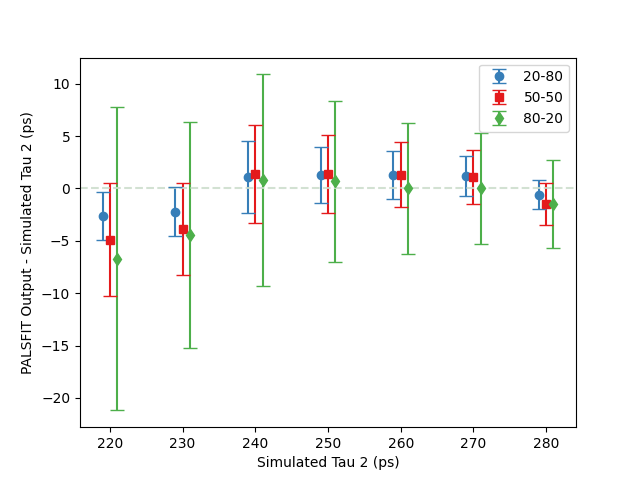
\includegraphics[width=.95\linewidth]{Batch 1+2/t2.png}
        \caption{$\tau_2$ difference}
        \label{fig:180-tau2}
    \end{subfigure}
    \begin{subfigure}{0.7\textwidth}
        \centering
        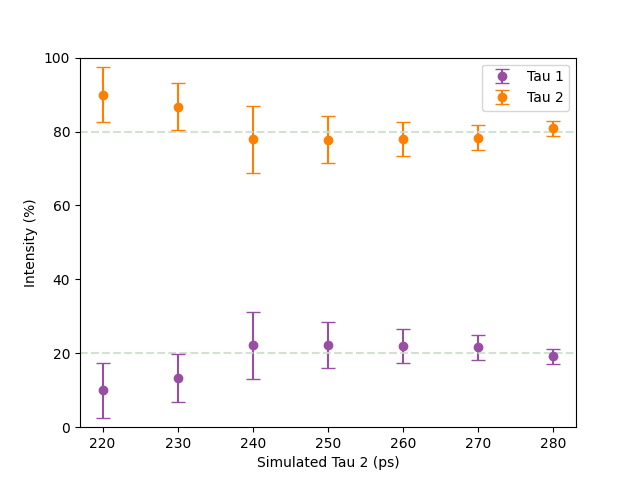
\includegraphics[width=.95\linewidth]{Batch 1+2/2080.png}
        \caption{$\tau_1 = 20\%, \tau_1 = 80\%$}
        \label{fig:180-2080}
    \end{subfigure}
    }
    \makebox[\linewidth][c]{
    \begin{subfigure}{.7\textwidth}
        \centering
        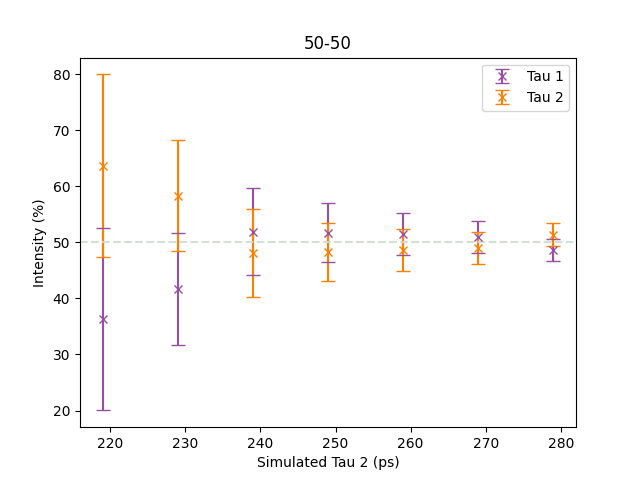
\includegraphics[width=0.95\linewidth]{Batch 1+2/5050.png}
        \caption{$\tau_1 = 50\%, \tau_2 = 50\%$}
        \label{fig:180-5050}
    \end{subfigure}
    \begin{subfigure}{.7\textwidth}
        \centering
        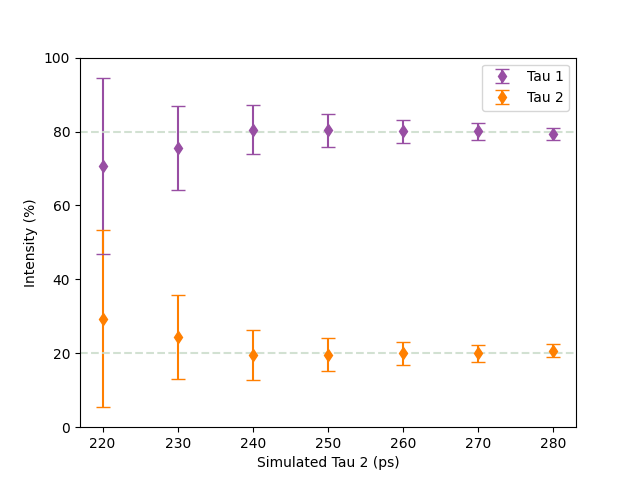
\includegraphics[width=0.95\linewidth]{Batch 1+2/8020.png}
        \caption{$\tau_1 = 80\%, \tau_2 = 20\%$}
        \label{fig:180-8020}
    \end{subfigure}
    }
\end{figure}

\pagebreak

\section{Modifying $\tau_1$}

A similar procedure was performed for $\tau_1$ = 150 and 220. To keep the relative time interval the same in between batches, the corresponding spacing between $\tau_1$ and the $\tau_2$ range was kept consistent. For $\tau_1$ = 150, this meant a $\tau_2$ range of 190-250ps, and for $\tau_1$ = 220, this meant a corresponding $\tau_2$ range of 260-320ps.

This was first done for $\tau_1$ = 150. As can be seen in Figures \ref{fig:150-tau1}-\ref{fig:150-8020}, the results for this batch are all within error, with both accuracy and precision getting better as the lifetime separation increases, in line with what would be expected.

The other batch, meanwhile, where $\tau_1$ was set to 220ps, was not as successful. The results can be seen in Figures \ref{fig:220-tau1}-\ref{fig:150-8020}, but in general, PALSFIT struggled with fitting the lowest values for $\tau_2$ and the error bars are noticably larger.

\todo{rewrite from here on properly}



\iffalse
As a point of comparison, $\tau_1$ was brought to 150 and the same analysis was performed. To keep things consistent, the $\tau_2$ range was modified to maintain the spacing between the lifetimes consistent between runs ($\tau_2$ = 180-250ps). In Figures \ref{fig:150-tau1}-\ref{fig:150-8020} we can see that the fitted values for $\tau_1$ and $\tau_2$ all fall within error of the original, simulated, values.
\fi

\begin{figure}[p]
    \centering
    \caption{}
    \makebox[\linewidth][c]{
        \begin{subfigure}{0.7\textwidth}
        \centering
        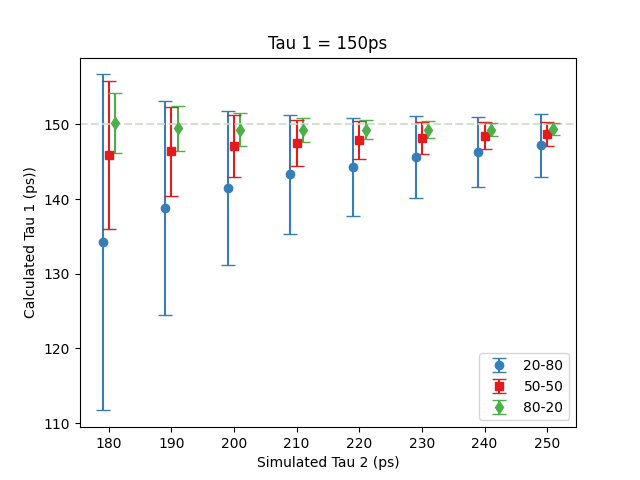
\includegraphics[width=0.95\linewidth]{Batch 3/regular IRF/tau1 150/output/t1.png}
        \caption{fixed $\tau_1 = 150ps$}
        \label{fig:150-tau1}
    \end{subfigure}
    \begin{subfigure}{0.7\textwidth}
        \centering
        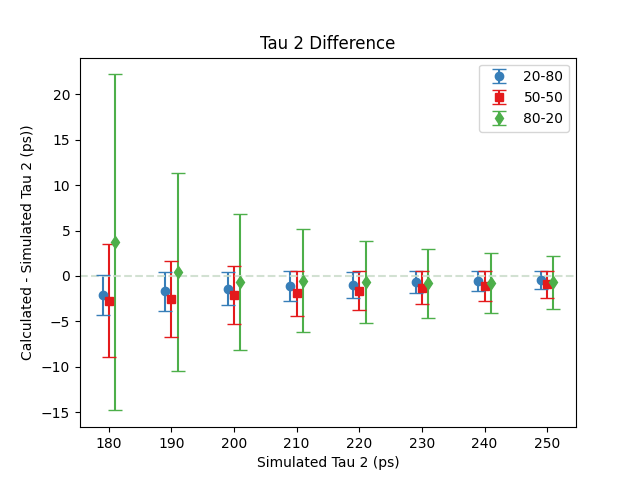
\includegraphics[width=.95\textwidth]{Batch 3/regular IRF/tau1 150/output/t2.png}
        \caption{$\tau_2$ difference}
        \label{fig:150-tau2}
    \end{subfigure}
    }
    \makebox[\linewidth][c]{
        \begin{subfigure}{0.7\textwidth}
        \centering
        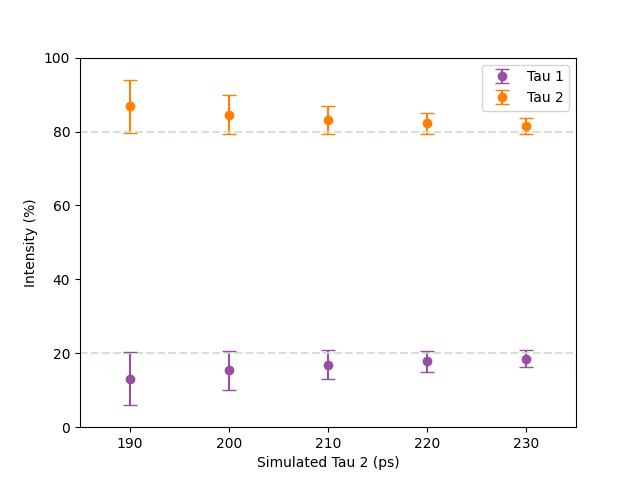
\includegraphics[width=0.95\linewidth]{Batch 3/regular IRF/tau1 150/output/2080r.png}
        \caption{$\tau_1 = 20\%, \tau_2 = 80\%$}
        \label{fig:150-2080}
    \end{subfigure}
    \begin{subfigure}{0.7\textwidth}
        \centering
        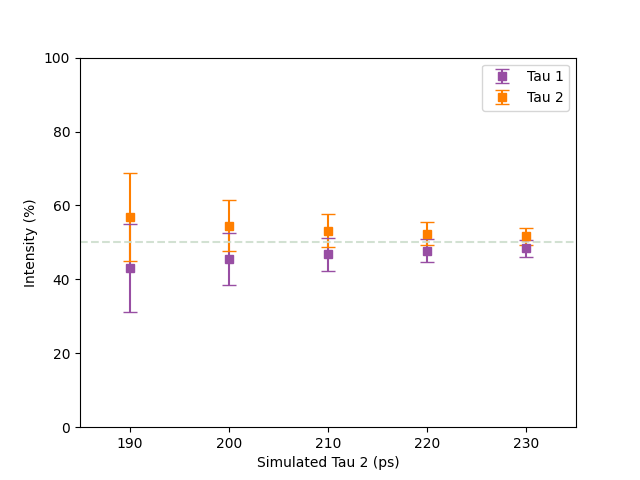
\includegraphics[width=.95\textwidth]{Batch 3/regular IRF/tau1 150/output/5050r.png}
        \caption{$\tau_1 = 50\%, \tau_2 = 50\%$}
        \label{fig:150-5050}
    \end{subfigure}
    }
    \begin{subfigure}{0.7\textwidth}
        \centering
        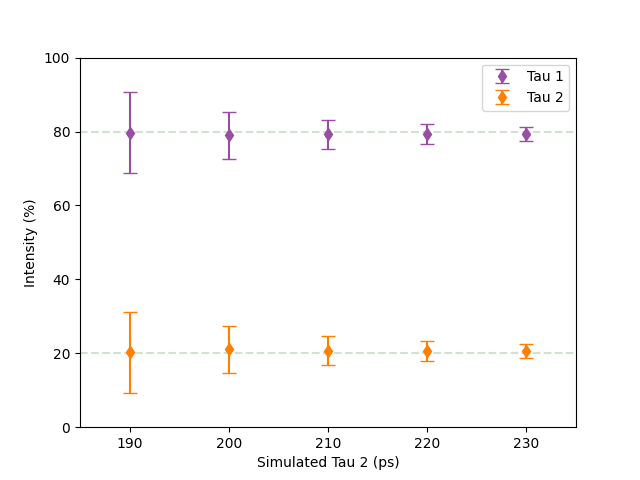
\includegraphics[width=.95\textwidth]{Batch 3/regular IRF/tau1 150/output/8020r.png}
        \caption{$\tau_1 = 80\%, \tau_2 = 20\%$}
        \label{fig:150-8020}
    \end{subfigure}
\end{figure}

\begin{figure}[p]
    \centering
    \caption{}
    \makebox[\linewidth][c]{
        \begin{subfigure}{0.7\textwidth}
        \centering
        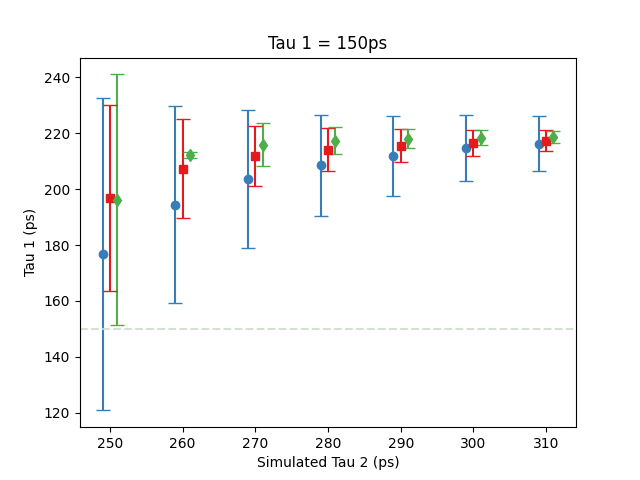
\includegraphics[width=0.95\linewidth]{Batch 3/regular IRF/tau1 220/output/t1.png}
        \caption{fixed $\tau_1 = 220ps$}
        \label{fig:220-tau1}
    \end{subfigure}
    \begin{subfigure}{0.7\textwidth}
        \centering
        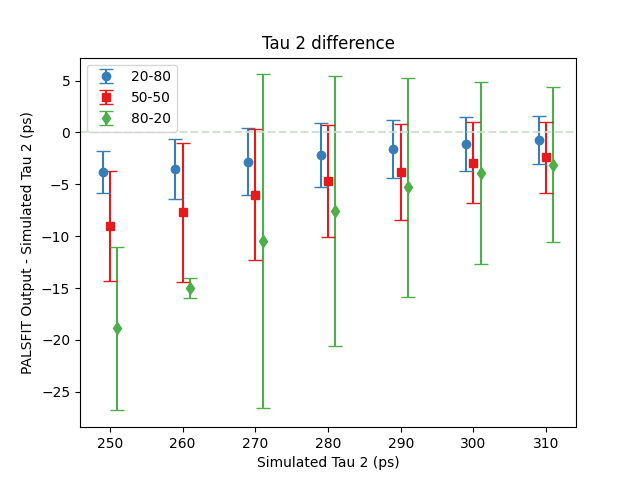
\includegraphics[width=.95\textwidth]{Batch 3/regular IRF/tau1 220/output/t2.png}
        \caption{$\tau_2$ difference}
        \label{fig:220-tau2}
    \end{subfigure}
    }
    \makebox[\linewidth][c]{
        \begin{subfigure}{0.7\textwidth}
        \centering
        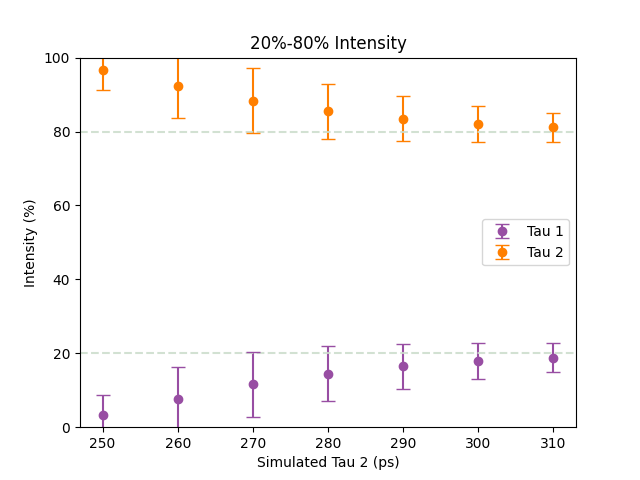
\includegraphics[width=0.95\linewidth]{Batch 3/regular IRF/tau1 220/output/2080.png}
        \caption{$\tau_1 = 20\%, \tau_2 = 80\%$}
        \label{fig:220-2080}
    \end{subfigure}
    \begin{subfigure}{0.7\textwidth}
        \centering
        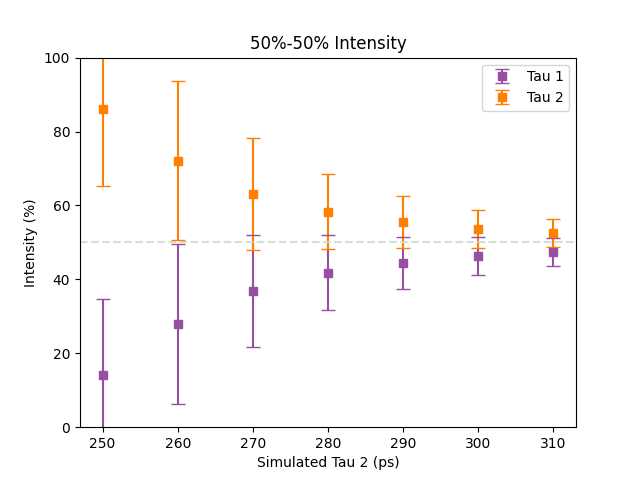
\includegraphics[width=.95\textwidth]{Batch 3/regular IRF/tau1 220/output/5050.png}
        \caption{$\tau_1 = 50\%, \tau_2 = 50\%$}
        \label{fig:220-5050}
    \end{subfigure}
    }
    \begin{subfigure}{0.7\textwidth}
        \centering
        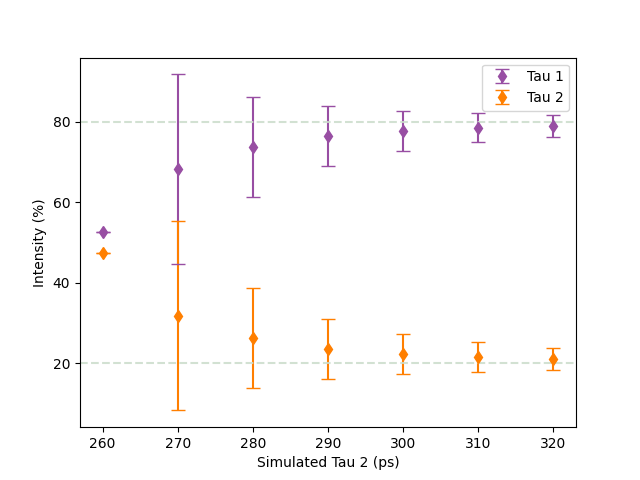
\includegraphics[width=.95\textwidth]{Batch 3/regular IRF/tau1 220/output/8020.png}
        \caption{$\tau_1 = 80\%, \tau_2 = 20\%$}
        \label{fig:220-8020}
    \end{subfigure}
\end{figure}

\begin{figure}[p]
    \centering
    \caption{$\tau_1$, rows = 20-80, 50-50, 80-20, columns = diff, std dev}    
    \makebox[\linewidth][c]{
        \begin{subfigure}{0.7\textwidth}
            \centering
            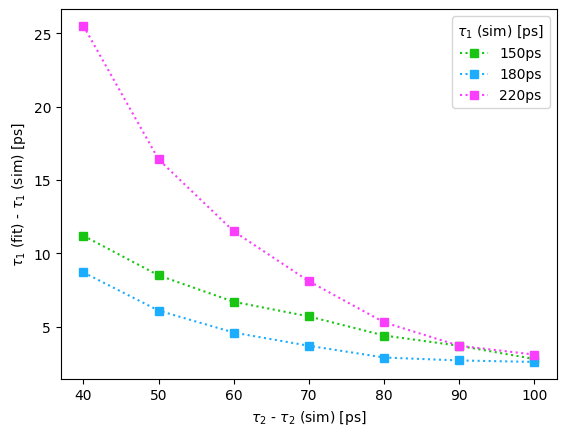
\includegraphics[width=0.95\linewidth]{Batch 3/regular IRF/t1-diff 2080.png}
            \label{fig:reg-t1-2080}
            \caption{}
        \end{subfigure}
        \begin{subfigure}{0.7\textwidth}
            \centering
            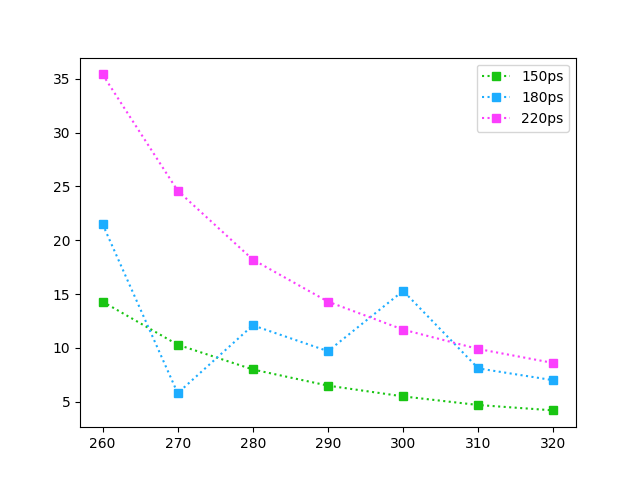
\includegraphics[width=0.95\linewidth]{Batch 3/regular IRF/t1-err 2080.png}
            \label{fig:reg-t1err-2080}
            \caption{}
        \end{subfigure}
    }

    \centering
    \makebox[\linewidth][c]{
        \begin{subfigure}{0.7\textwidth}
            \centering
            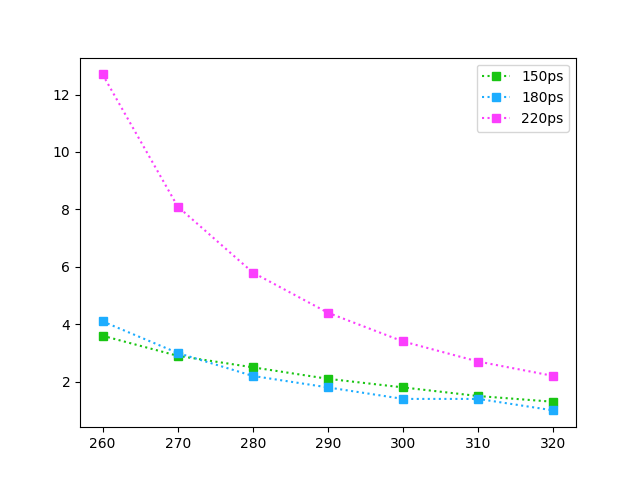
\includegraphics[width=0.95\linewidth]{Batch 3/regular IRF/t1-diff 5050.png}
            \label{fig:reg-t1-5050}
            \caption{}
        \end{subfigure}
        \begin{subfigure}{0.7\textwidth}
            \centering
            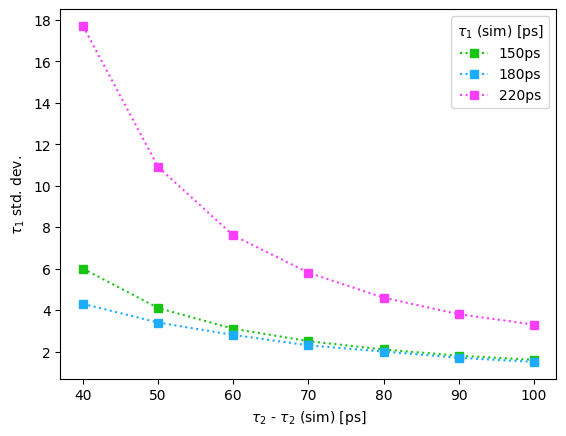
\includegraphics[width=0.95\linewidth]{Batch 3/regular IRF/t1-err 5050.png}
            \label{fig:reg-t1err-5050}
            \caption{}
        \end{subfigure}
    }

    \centering
    \makebox[\linewidth][c]{
        \begin{subfigure}{0.7\textwidth}
            \centering
            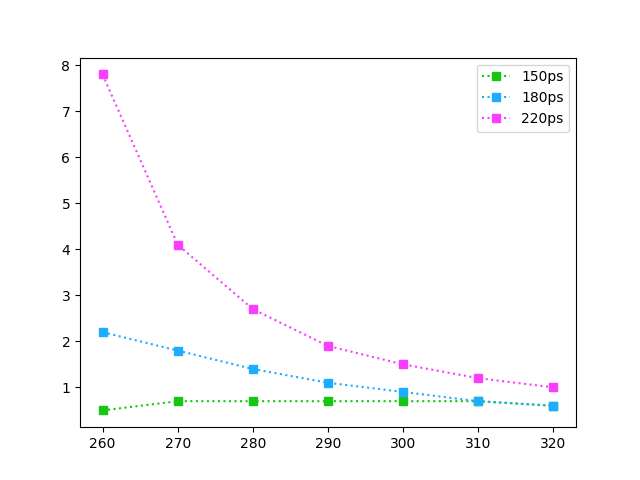
\includegraphics[width=0.95\linewidth]{Batch 3/regular IRF/t1-diff 8020.png}
            \label{fig:reg-t1-8020}
            \caption{}
        \end{subfigure}
        \begin{subfigure}{0.7\textwidth}
            \centering
            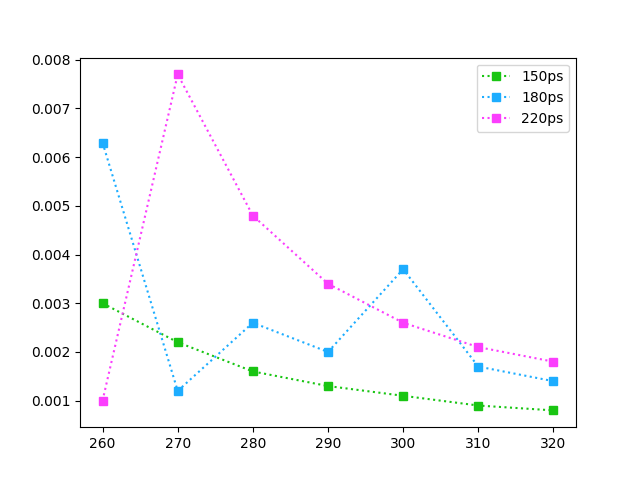
\includegraphics[width=0.95\linewidth]{Batch 3/regular IRF/t1-err 8020.png}
            \label{fig:reg-t1err-8020}
            \caption{}
        \end{subfigure}
    }
\end{figure}

\begin{figure}[p]
    \centering
    \caption{$\tau_2$, rows = 20-80, 50-50, 80-20, columns = diff, std dev}
    \makebox[\linewidth][c]{
        \begin{subfigure}{0.7\textwidth}
            \centering
            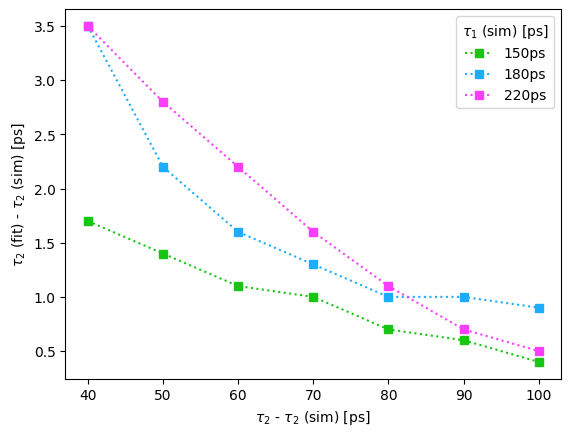
\includegraphics[width=0.95\linewidth]{Batch 3/regular IRF/t2-diff 2080.png}
            \label{fig:reg-t2-2080}
            \caption{}
        \end{subfigure}
        \begin{subfigure}{0.7\textwidth}
            \centering
            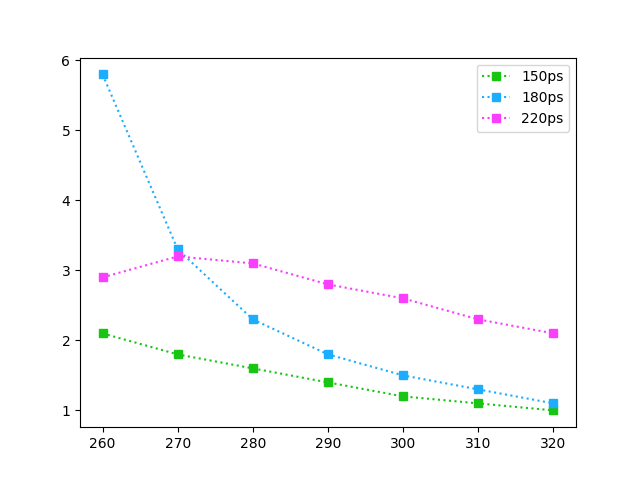
\includegraphics[width=0.95\linewidth]{Batch 3/regular IRF/t2-err 2080.png}
            \label{fig:reg-t2err-2080}
            \caption{}
        \end{subfigure}
    }

    \centering
    \makebox[\linewidth][c]{
        \begin{subfigure}{0.7\textwidth}
            \centering
            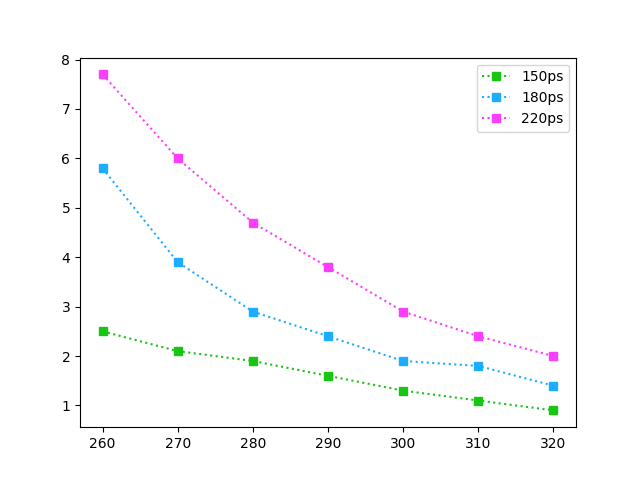
\includegraphics[width=0.95\linewidth]{Batch 3/regular IRF/t2-diff 5050.png}
            \label{fig:reg-t2-5050}
            \caption{}
        \end{subfigure}
        \begin{subfigure}{0.7\textwidth}
            \centering
            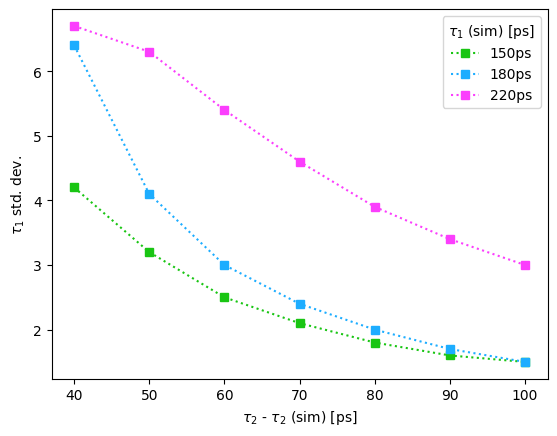
\includegraphics[width=0.95\linewidth]{Batch 3/regular IRF/t2-err 5050.png}
            \label{fig:reg-t2err-5050}
            \caption{}
        \end{subfigure}
    }

    \centering
    \makebox[\linewidth][c]{
        \begin{subfigure}{0.7\textwidth}
            \centering
            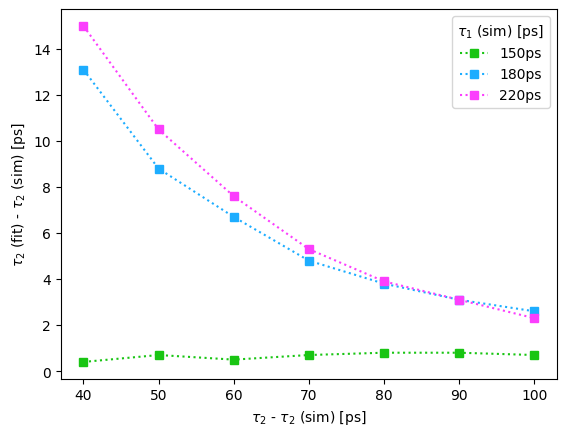
\includegraphics[width=0.95\linewidth]{Batch 3/regular IRF/t2-diff 8020.png}
            \label{fig:reg-t2-8020}
            \caption{}
        \end{subfigure}
        \begin{subfigure}{0.7\textwidth}
            \centering
            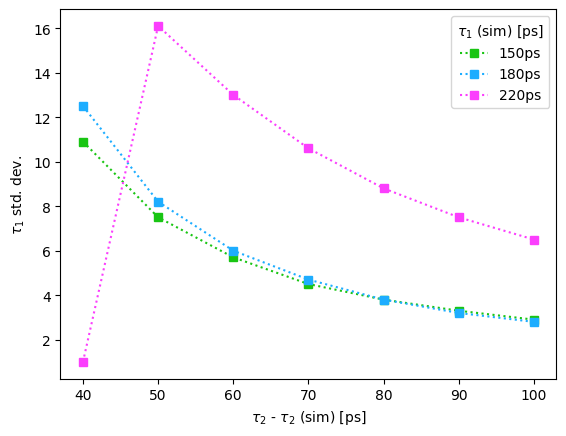
\includegraphics[width=0.95\linewidth]{Batch 3/regular IRF/t2-err 8020.png}
            \label{fig:reg-t2err-8020}
            \caption{}
        \end{subfigure}
    }
        
\end{figure}

\begin{figure}[p]
    \centering
    \caption{intensities, rows = 20-80, 50-50, 80-20, columns = diff, std dev}
    \makebox[\linewidth][c]{
        \begin{subfigure}{0.7\textwidth}
            \centering
            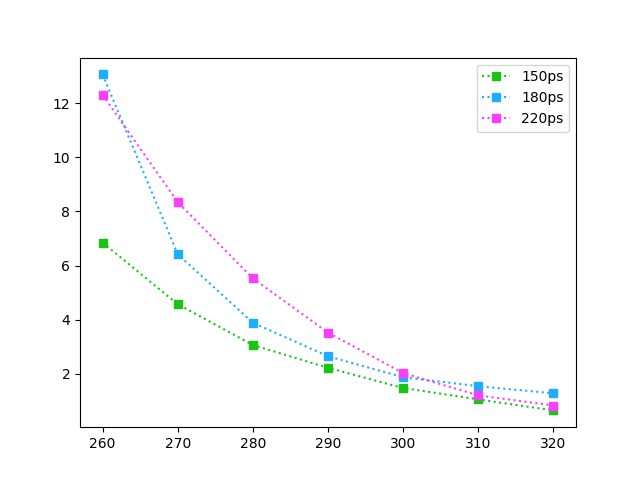
\includegraphics[width=0.95\linewidth]{Batch 3/regular IRF/2080-diff i1.png}
            \label{fig:reg-int-2080}
            \caption{}
        \end{subfigure}
        \begin{subfigure}{0.7\textwidth}
            \centering
            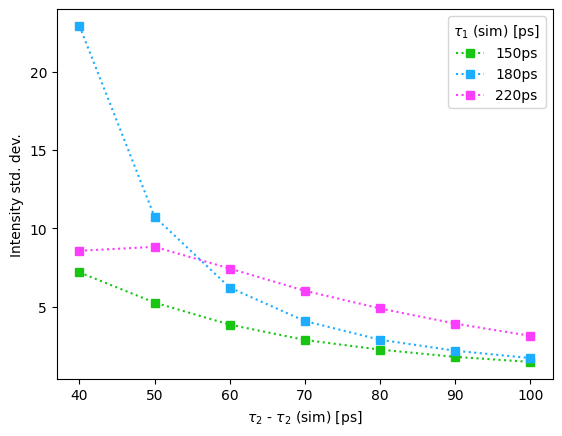
\includegraphics[width=0.95\linewidth]{Batch 3/regular IRF/2080-err i1.png}
            \label{fig:reg-interr-2080}
            \caption{}
        \end{subfigure}
    }

    \centering
    \makebox[\linewidth][c]{
        \begin{subfigure}{0.7\textwidth}
            \centering
            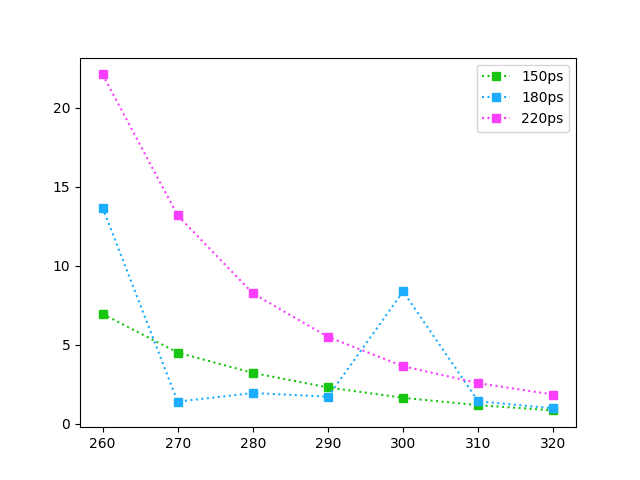
\includegraphics[width=0.95\linewidth]{Batch 3/regular IRF/5050-diff i1.png}
            \label{fig:reg-int-5050}
            \caption{}
        \end{subfigure}
        \begin{subfigure}{0.7\textwidth}
            \centering
            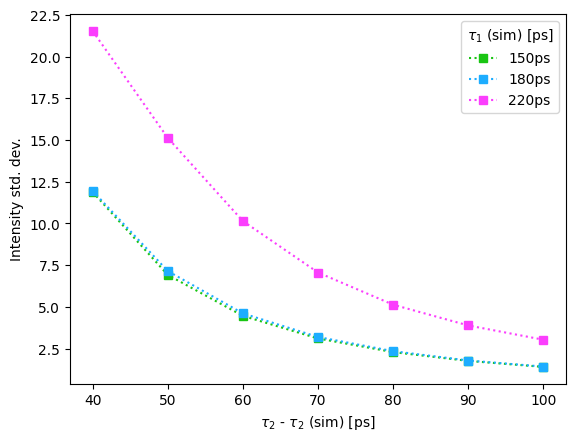
\includegraphics[width=0.95\linewidth]{Batch 3/regular IRF/5050-err i1.png}
            \label{fig:reg-interr-5050}
            \caption{}
        \end{subfigure}
    }

    \centering
    \makebox[\linewidth][c]{
        \begin{subfigure}{0.7\textwidth}
            \centering
            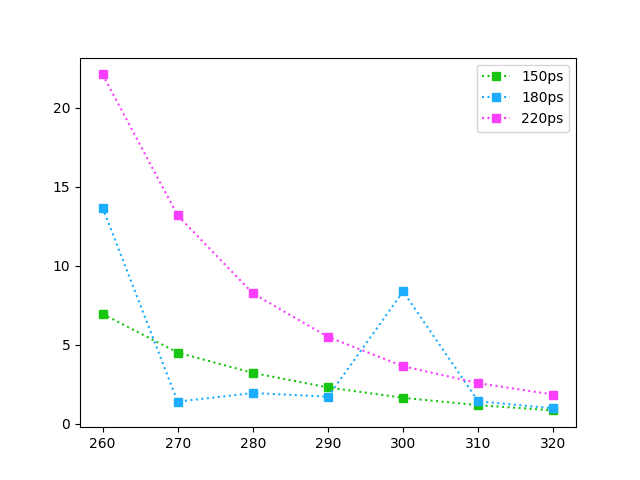
\includegraphics[width=0.95\linewidth]{Batch 3/regular IRF/5050-diff i1.png}
            \label{fig:reg-int-8020}
            \caption{}
        \end{subfigure}
        \begin{subfigure}{0.7\textwidth}
            \centering
            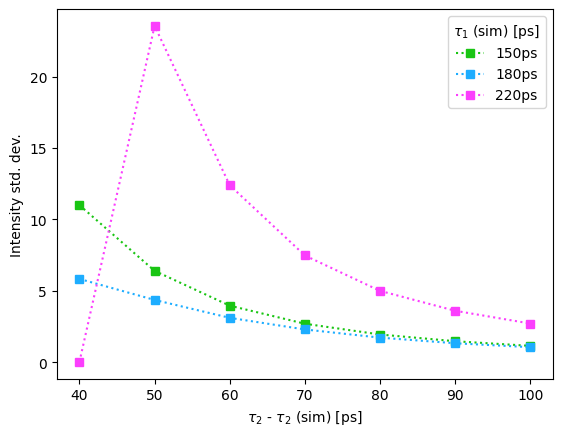
\includegraphics[width=0.95\linewidth]{Batch 3/regular IRF/8020-err i1.png}
            \label{fig:reg-interr-8020}
            \caption{}
        \end{subfigure}
    }
        
\end{figure}

\pagebreak

\section{Instrument resolution function}

Using Python, we can plot the three gaussian functions that compose the instrument resolution function. The equation for a Gaussian function with parameters $a$, $b$ and $c$ (corresponding to the height of the peak, the position of the peak and the width of the graph) is given by the equation:

\[g(x) = a\exp{\left(-\frac{(x-b)^2}{2c^2}\right)} \]

While $a$ and $b$ map easily to the intensity and shift columns in Table \ref{tab:irf} ,  $c$ is expressed as a standard deviation, and not the full-half-width-maximum given in the table. To convert from one to the other, we can use the following expression:

\[ FWHM = 2\sqrt{2\ln(2)} \approx 2.355c \]

The resultant resolution function is, then, just the sum of the three gaussians $g_s(x)$, where

\[g_s(x) = \sum_{i=1}^{3}{a_i \exp{\left(-\frac{(x-b)^2}{2c^2}\right)}}\]

This resolution function looks quite similar to a gaussian function itself, and thus it seems sensible to investigate the feasability of approximating a more complex 3 gaussian resolution function, with a single gaussian.

The intensity of the single gaussian approximation is the easiest parameter to determine, as it's simply 100\%. We could try to determine $b$ and $c$ analytically by solving the resulting $g_s(x)$ analytically, but, as we already have already generated a list of values for $g_s(x)$ when plotting the function, it's much easier to just extract the needed values numerically using Python.

Finding $b$ is as easy as finding the largest element of the list, and its corresponding $x$ value. As PALSSIM requires the FWHM rather than the standard deviation $c$, we just need to find the difference between the two values of $x$ for which $g_s(x)$ is closest to half of the IRF.

Doing so gives us the following values to insert into PALSSIM:

\begin{table}[h]
    \centering
    \begin{tabular}{|c|c|c|}
        \hline
        FWHM (ps) &  Shift (ps) & Intensity (\%) \\
        \hline
        210 & 0 & 100\\ 
        \hline
    \end{tabular}
    \caption{Single gaussian Instrument resolution function}
    \label{tab:irf-single}
\end{table}

Plugging in these values into PALSSIM gives us very similar results to the three gaussian IRF, with slight differences in the first datapoint for some of the graphs. Overall, though, it does seems like we can reasonably approximate a more complex, three gaussian IRF with a single gaussian.

The next step would be to examine how the width of the instrument resolution function (IRF) affects the results. The values for $\tau_1$ and $\tau_2$ can be set to be kept the same between runs, with $\tau_1$ fixed to 150ps and $\tau_2$ ranging from 180-230ps, as we had the best results with these values. The full-width half maximum of our single gaussian IRF can be set to the following values: 100ps, 150ps, 180ps, 210ps.

